\documentclass{beamer}
\usetheme{Madrid}
\usepackage{tikz}
\usepackage{booktabs}
\usetikzlibrary{positioning}
\title{Designing Markets: Chapter 4 Summary}
\subtitle{Handbook of Market Design}
\author{Your Name \& Partner Name}
\date{\today}

\begin{document}

% Slide 1: Title
\begin{frame}
    \titlepage
\end{frame}

% Slide 2: What is Market Design?
\begin{frame}{What is Market Design?}
    \begin{itemize}
        \item Market design creates rules and procedures for transactions.
        \item It aims to solve failures in existing or new markets.
        \item Success is measured by efficient, fair outcomes.
    \end{itemize}
    \vspace{0.4em}
    \begin{block}{Quick Example}
        Kidney exchange programs match donors and recipients who are incompatible within pairs.
    \end{block}
\end{frame}

% Slide 3: The Three Pillars
\begin{frame}{Three Pillars of Market Design}
    \begin{itemize}
        \item Thickness: Many participants at once.
        \item Safety: Truthful participation is encouraged.
        \item Congestion: Transactions are processed efficiently.
    \end{itemize}
    \vspace{0.6em}
    \centering
    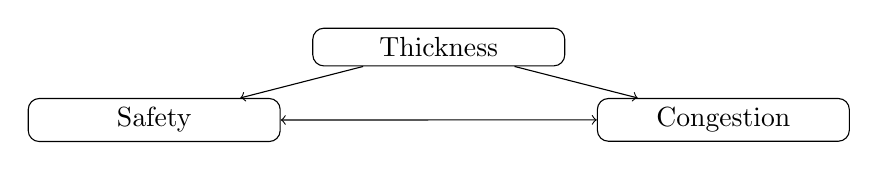
\begin{tikzpicture}[node distance=1.2cm, every node/.style={draw, rounded corners, align=center, minimum width=3.2cm}]
        \node (t) {Thickness};
        \node (s) [below left=0.4cm and 0.4cm of t] {Safety};
        \node (c) [below right=0.4cm and 0.4cm of t] {Congestion};
        \draw[->] (t) -- (s);
        \draw[->] (t) -- (c);
        \draw[<->] (s) -- (c);
    \end{tikzpicture}
\end{frame}

% Slide 4: Diagnosing Market Failures
\begin{frame}{Diagnosing Market Failures}
    \begin{itemize}
        \item Failures often result from poor timing or rules.
        \item Congestion and lack of thickness are common issues.
        \item Example: Residency match programs before redesign.
    \end{itemize}
    \vspace{0.4em}
    \begin{block}{Symptoms}
        Early contracting, thin participation, and strategic misreporting.
    \end{block}
    \vspace{0.2em}
    \centering
    \begin{tabular}{@{}ll@{}}
        \toprule
        Symptom & Likely Cause \\
        \midrule
        Early offers & Timing pressure \\
        Low participation & Thin market \\
        Strategic ranking & Unsafe rules \\
        \bottomrule
    \end{tabular}
\end{frame}

% Slide 5: Real-World Applications
\begin{frame}{Real-World Applications}
    \begin{itemize}
        \item Medical residency matches (NRMP)
        \item Public school choice systems
        \item Kidney exchanges
    \end{itemize}
    \vspace{0.6em}
    \centering
    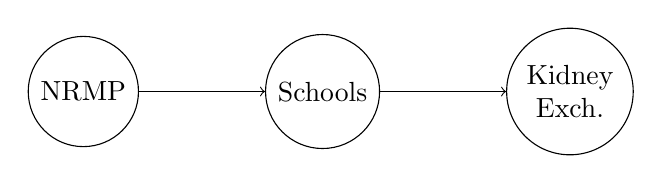
\begin{tikzpicture}[every node/.style={draw, circle, minimum size=1.2cm, align=center}]
        \node (a) {NRMP};
        \node (b) [right=1.6cm of a] {Schools};
        \node (c) [right=1.6cm of b] {Kidney\\Exch.};
        \draw[->] (a) -- (b);
        \draw[->] (b) -- (c);
    \end{tikzpicture}
\end{frame}

% Slide 6: Evaluating and Comparing Designs
\begin{frame}{Evaluating and Comparing Designs}
    \begin{itemize}
        \item Mechanism stability and outcome efficiency are key.
        \item Stable designs prevent market unraveling.
        \item Efficiency ensures resources are well allocated.
    \end{itemize}
    \vspace{0.4em}
    \centering
    \begin{tabular}{lcc}
        \toprule
        Criterion & Stable? & Efficient? \\
        \midrule
        Deferred Acceptance & Yes & Yes \\
        First-come-first-served & No & No \\
        \bottomrule
    \end{tabular}
    \vspace{0.5em}
    \begin{block}{Evaluation Checklist}
        Strategy-proofness, fairness (no justified envy), and simplicity for participants.
    \end{block}
\end{frame}

% Slide 7: Mechanism Stability
\begin{frame}{Mechanism Stability}
    \begin{itemize}
        \item A matching is stable if no pair prefers each other over current matches.
        \item Stability is crucial for long-term market health.
    \end{itemize}
    \vspace{0.4em}
    \begin{block}{Why it matters}
        Instability encourages participants to bypass the mechanism.
    \end{block}
\end{frame}

% Slide 8: Conclusion
\begin{frame}{Conclusion}
    \begin{itemize}
        \item Effective market design requires diagnosis and iteration.
        \item AI tools help simulate and verify market rules.
    \end{itemize}
    \vspace{0.4em}
    \begin{block}{Takeaway}
        Good design aligns incentives, improves participation, and reduces congestion.
    \end{block}
\end{frame}

% Slide 9: Exercise 1 (Manual Workflow)
\begin{frame}{Exercise 1: Manual Workflow}
    \begin{itemize}
        \item Collaborator manually updates "Diagnosing Market Failures" slide.
        \item Follow GitHub workflow: branch, comment, pull request, merge.
    \end{itemize}
\end{frame}

% Slide 10: Exercise 2 (AI Workflow)
\begin{frame}{Exercise 2: AI Workflow}
    \begin{itemize}
        \item Collaborator uses AI agent to update "Evaluating and Comparing Designs" slide.
        \item AI agent performs branch, comment, pull request, and merge.
    \end{itemize}
\end{frame}

\end{document}
